% ============================================================
% GSPH-FC (v3) — Springer LNCS — VERSIÓN EN ESPAÑOL
% Traducción de samplepaper_v3.tex (mismos datos, tablas y figuras).
% Compilar: pdflatex -> bibtex -> pdflatex -> pdflatex
% Figuras: Resultados_v2/ (tours) y Resultados_v3/ (convergencia)
% Cómo regenerar cada tabla y figura: REPRODUCIR.md
% ============================================================
\documentclass[runningheads]{llncs}
\usepackage[T1]{fontenc}
\usepackage[utf8]{inputenc}
\usepackage[spanish,es-tabla,es-noshorthands,es-nodecimaldot]{babel}
\usepackage{graphicx}
\usepackage{amsmath,amssymb}
\usepackage{booktabs}
\usepackage{algorithm}
\usepackage[noend]{algpseudocode}
\usepackage{url}

\floatname{algorithm}{Algoritmo}
\algrenewcommand\algorithmicrequire{\textbf{Entrada:}}
\algrenewcommand\algorithmicensure{\textbf{Salida:}}
\algrenewcommand\algorithmicwhile{\textbf{mientras}}
\algrenewcommand\algorithmicdo{\textbf{hacer}}
\algrenewcommand\algorithmicforall{\textbf{para todo}}
\algrenewcommand\algorithmicif{\textbf{si}}
\algrenewcommand\algorithmicthen{\textbf{entonces}}
\algrenewcommand\algorithmicelse{\textbf{si no}}
\algrenewcommand\algorithmicreturn{\textbf{devolver}}
\AtBeginDocument{\renewcommand\keywordname{{\bfseries Palabras clave:}}}

\begin{document}

\title{GSPH-FC: partición geométrica con conectividad de fronteras
y búsqueda local iterada localizada para el TSP euclidiano}
\titlerunning{GSPH-FC para el TSP euclidiano}

\author{%
    Martín Gómez Navarro\inst{1} \and
    Rodrigo Linfati\inst{2} \and
    Juan Carlos Figueroa-García\inst{3} \and
    Carlos Alberto Franco Franco\inst{3} \and
    Daniel Morillo-Torres\inst{4} \and
    Jairo R. Coronado-Hernandez\inst{5} \and
    Gustavo Esteban Gatica\inst{1}}
\authorrunning{M. Gómez Navarro et al.}
\institute{%
    Facultad de Ingeniería, Universidad Andrés Bello, Santiago, Chile\\
    \email{m.gmeznavarro@uandresbello.edu}\\
    \email{ggatica@uandresbello.edu}
    \and
    Facultad de Ingeniería, Universidad del Bío-Bío,
    Concepción, Chile\\
    \email{rlinfati@ubiobio.cl}
    \and
    Facultad de Ingeniería, Universidad Distrital
    Francisco José de Caldas, Bogotá, Colombia\\
    \email{jcfigueroag@udistrital.edu.co}
    \email{cafrancof@udistrital.edu.co}
    \and
    Facultad de Ingeniería, Pontificia Universidad Javeriana de Cali,
    Cali, Colombia\\
    \email{daniel.morillo@javerianacali.edu.co}
    \and
    Facultad de Ingeniería, Universidad de la Costa,
    Barranquilla, Colombia\\
    \email{jcoronad18@cuc.edu.co}}

\maketitle

\begin{abstract}
Presentamos \textbf{GSPH-FC}, una heurística para el problema del
vendedor viajero (TSP) euclidiano formada por dos partes. La primera es
una construcción geométrica: el plano se divide en cuatro cuadrantes,
las conexiones entre cuadrantes vecinos (pares de frontera) se eligen
\emph{antes} de que exista cualquier ruta local, y luego cada cuadrante
se recorre con un camino abierto anclado en esas conexiones. La segunda
es una búsqueda local iterada (ILS) localizada: 2-opt y Or-opt con
listas de vecinos, un double-bridge confinado a una ventana que crece con
el tamaño de la instancia, aceptación de Metropolis, deshacer mediante un
registro de inversiones de segmentos y parada por estancamiento, todo
compilado a código nativo. En 77 instancias de TSPLIB de hasta 18\,512
ciudades, GSPH-FC alcanza la mejor solución conocida (BKS) en 44,
incluidas las 36 instancias con $n\le 300$ en menos de 0.5~s cada una, y
su mejor tour queda a menos de 0.60\% de la BKS hasta 6\,000 ciudades.
Más allá del benchmark, medimos de dónde viene esa calidad. Una ablación
con el motor de búsqueda fijo muestra que la conectividad de fronteras
entrega los mejores tours iniciales (9.95\% sobre la BKS frente a
24.71\% del vecino más cercano) y la mayor cantidad de aciertos de la
BKS, mientras que el ILS localizado explica la mayor parte de la calidad
final. Las curvas de convergencia en el tiempo no muestran una ventaja
temprana de la construcción completa, que paga un costo inicial: el ILS
borra la mayor parte de las diferencias entre tours iniciales dentro de
la primera décima de la ejecución, y los inicios geométricos ayudan sobre
todo a evitar zonas pobres del espacio de búsqueda, como aquellas en que
cae el vecino más cercano en instancias agrupadas. Un estudio de
sensibilidad en 16 instancias y una comparación con LKH-3 sitúan a
GSPH-FC como una heurística liviana e interpretable: iguala a LKH en
instancias pequeñas, pero es menos precisa por encima de 300 ciudades.
\keywords{Problema del vendedor viajero \and Descomposición geométrica
\and Conectividad de fronteras \and Búsqueda local iterada \and 2-opt
\and TSPLIB}
\end{abstract}

% ================================================================
\section{Introducción}
% ================================================================

El \textit{problema del vendedor viajero} (TSP) euclidiano busca el
ciclo hamiltoniano más corto que pase por $n$ puntos del plano. Es un
banco de prueba clásico para el diseño de heurísticas en optimización
combinatoria~\cite{applegate2006tsp,laporte1992tsp}, y las heurísticas
siguen siendo útiles cuando un método debe ser rápido, simple de
implementar y fácil de explicar, más que óptimo a cualquier
costo~\cite{garey1979computers,mardones2023}.

En el caso euclidiano, la geometría es la estructura evidente para
aprovechar, y los métodos basados en particiones lo hacen dividiendo el
plano, resolviendo cada región y uniendo las piezas. En la mayoría de
ellos las uniones son algo secundario: los subtours se parchan, las fija
el orden de una curva o se heredan de un tour previo. \textbf{GSPH-FC}
(\textit{Geometric Space Partitioning with Frontier Connectivity}) parte
de la idea opuesta: las conexiones entre regiones se deciden primero, a
partir de la geometría de las fronteras, y luego las rutas dentro de cada
región se construyen respetándolas. El tour resultante se mejora con un
ILS localizado, diseñado para que cada iteración cueste microsegundos.

Una heurística con una fase constructiva y una de mejora plantea una
pregunta obvia: ¿cuánto de la calidad final se debe a cada una? Un motor
de mejora fuerte puede hacer que casi cualquier tour inicial parezca
bueno, lo que volvería irrelevante a la construcción. Por eso no nos
quedamos en los resultados del benchmark: medimos directamente el aporte
de cada fase.

\paragraph{Contribuciones.}
\begin{enumerate}
  \item \textbf{Una construcción geométrica condicionada por fronteras.}
    Los pares de frontera entre cuadrantes vecinos se eligen antes del
    ruteo local y se imponen como extremos fijos de caminos anclados
    dentro de cada cuadrante, evaluados sobre un pequeño portafolio de
    particiones y combinaciones de fronteras.
  \item \textbf{Un motor ILS localizado.} Una perturbación double-bridge
    confinada a una ventana que depende del tamaño, aceptación de
    Metropolis, deshacer repitiendo las inversiones registradas en vez de
    copiar el tour y parada por estancamiento, implementados como núcleos
    compilados sobre arreglos de índices.
  \item \textbf{Un análisis de dónde viene la calidad.} Una ablación de la
    construcción con el motor fijo, curvas de convergencia del mejor tour
    en el tiempo, un estudio de sensibilidad de parámetros en 16
    instancias de distintos tamaños y distribuciones espaciales, y una
    comparación con LKH-3, junto con scripts que reproducen cada tabla y
    figura.
\end{enumerate}

La Sección~\ref{sec:related} revisa el trabajo relacionado, la
Sección~\ref{sec:method} describe la construcción y la
Sección~\ref{sec:engine} el motor de mejora y su complejidad. La
Sección~\ref{sec:setup} presenta la configuración experimental, la
Sección~\ref{sec:results} los resultados, la
Sección~\ref{sec:discussion} los discute y la
Sección~\ref{sec:conclusions} concluye.

% ================================================================
\section{Trabajo relacionado}
\label{sec:related}
% ================================================================

\paragraph{Construcción y búsqueda local.} El vecino más cercano (NN) es
la línea base constructiva clásica: corre en $O(n^2)$ y se usa a menudo
como punto de partida de heurísticas de mejora, pero por sí solo queda
lejos del óptimo~\cite{kizilatecs2013nearest}. El movimiento 2-opt
invierte un segmento cuando eso acorta el tour~\cite{croes1958method};
con listas de candidatos y don't-look bits es un componente básico de la
búsqueda local euclidiana~\cite{johnson1997tsp,bentley1992fast}. Or-opt
reubica segmentos cortos y complementa a 2-opt a bajo
costo~\cite{or1976traveling}. La familia Lin--Kernighan, y en particular
LKH, extienden estas ideas a movimientos de profundidad variable y están
entre las heurísticas prácticas más fuertes para el
TSP~\cite{lin1973effective,helsgaun2000effective,helsgaun2017extension}.

\paragraph{Búsqueda local iterada.} El ILS alterna perturbación y
búsqueda local para escapar de óptimos locales~\cite{lourencco2003ils}.
En el TSP, el double-bridge seguido de reoptimización local es una
combinación especialmente efectiva. Las cadenas de Markov de paso largo
de Martin, Otto y Felten aceptan tours peores con una probabilidad tipo
Boltzmann~\cite{martin1991large}, como en el recocido
simulado~\cite{kirkpatrick1983optimization}. Nuestro motor pertenece a
esta línea; lo distinguen el confinamiento de la perturbación a una
ventana y el registro de inversiones que abarata deshacer las
perturbaciones rechazadas.

\paragraph{Descomposición geométrica.} El algoritmo de partición de Karp
divide el plano recursivamente en celdas, resuelve cada celda y une los
subtours, con garantías probabilísticas para puntos
uniformes~\cite{karp1977probabilistic}. Las heurísticas de curvas que
llenan el espacio visitan los puntos en el orden de una curva recursiva
por cuadrantes en tiempo $O(n\log n)$~\cite{bartholdi1982spacefilling}.
POPMUSIC descompone un tour existente en subproblemas superpuestos que se
reoptimizan por separado, y lo usa para construir listas de candidatos
para LKH~\cite{taillard2019popmusic}. En los tres, las conexiones entre
regiones son un subproducto de la unión de subtours, del orden de una
curva o de un tour previo. En GSPH-FC son una decisión explícita, tomada
antes de rutear las regiones.

\begin{table}
\caption{Principales familias de métodos para el TSP y sus compromisos
cualitativos.}
\label{tab:comparison}
\centering\small
\begin{tabular}{@{}lllll@{}}
\toprule
\textbf{Método} & \textbf{Tipo} & \textbf{Complejidad} & \textbf{Escalabilidad} & \textbf{Calidad} \\
\midrule
Fuerza bruta          & Exacto        & $O(n!)$      & Muy baja  & Óptima \\
Programación dinámica & Exacto        & $O(n^2 2^n)$ & Baja      & Óptima \\
Vecino más cercano    & Constructivo  & $O(n^2)$     & Alta      & Baja \\
2-opt                 & Mejora        & $O(n^2)$/iter& Media     & Media \\
Lin--Kernighan/LKH    & Mejora        & Variable     & Alta      & Muy alta \\
Heurísticas tipo ILS  & Metaheurística & Variable    & Alta      & Alta \\
\textbf{GSPH-FC}      & Geométrica + ILS & $O(n^2)+K$ iter.$^{*}$ & Alta & Alta \\
\bottomrule
\multicolumn{5}{@{}l}{\scriptsize $^{*}$Construcción más $K$ iteraciones de ILS; ver Sección~\ref{sec:complexity}.}
\end{tabular}
\end{table}

% ================================================================
\section{Construcción geométrica condicionada por fronteras}
\label{sec:method}
% ================================================================

\subsection{Problema}

Sea $V=\{v_1,\dots,v_n\}\subset\mathbb{R}^2$ con coordenadas
$(x_i,y_i)$, y sean los costos de las aristas los de la convención
\texttt{EUC\_2D} de TSPLIB~\cite{reinelt1991tsplib}:
\begin{equation}
 d(v_i,v_j)=\left\lfloor\sqrt{(x_i-x_j)^2+(y_i-y_j)^2}+0.5\right\rfloor.
 \label{eq:dist}
\end{equation}
El TSP busca una permutación cíclica $\pi$ que minimice
\begin{equation}
 L(\pi)=\sum_{i=1}^{n} d\!\left(v_{\pi(i)},v_{\pi(i\bmod n+1)}\right).
 \label{eq:tsp}
\end{equation}
Todos los GAP de este trabajo se calculan contra valores de BKS en la
misma métrica.

\subsection{Descomposición geométrica}

Para un punto de corte $(x_m,y_m)$, los puntos se dividen en cuatro
cuadrantes:
\begin{align}
Q_1&=\{v: x_v\le x_m,\; y_v>y_m\}  &&\text{(NO)}, &
Q_2&=\{v: x_v>x_m,\; y_v>y_m\}    &&\text{(NE)},\\
Q_3&=\{v: x_v\le x_m,\; y_v\le y_m\}&&\text{(SO)}, &
Q_4&=\{v: x_v>x_m,\; y_v\le y_m\} &&\text{(SE)}.
\end{align}
En vez de un solo punto de corte, el método evalúa un pequeño portafolio
de tres a cinco (menos para $n$ grande): el punto medio de la caja
envolvente, la mediana por coordenada y cuatro puntos medios de la caja
desplazados en un 12\% de su lado hacia cada diagonal.

\subsection{Conectividad de fronteras}

Cada par de cuadrantes vecinos $Q_a,Q_b$ comparte una frontera, ya sea la
recta $x=x_m$ o la recta $y=y_m$. Para una frontera vertical, las bandas
de frontera son
\begin{equation}
F_a(\varepsilon)=\{u\in Q_a:|x_u-x_m|<\varepsilon\}, \qquad
F_b(\varepsilon)=\{v\in Q_b:|x_v-x_m|<\varepsilon\},
\end{equation}
y el mejor par de frontera es
\begin{equation}
(u^*,v^*)=\arg\min_{u\in F_a,\,v\in F_b} d(u,v).
\label{eq:frontier}
\end{equation}
Si una banda está vacía, $\varepsilon$ se duplica hasta cuatro veces. El
método guarda los tres mejores pares de cada una de las cuatro fronteras
y ordena sus combinaciones por el largo total de frontera. Cada
combinación elegida fija, para cada cuadrante, un punto de entrada (el
nodo donde llega el tour desde el cuadrante anterior) y un punto de
salida (el nodo desde donde sale hacia el siguiente).

\subsection{Caminos anclados dentro de cada cuadrante}

Dado un cuadrante $Q_k$ con entrada $s_k$ y salida $t_k$, su ruta es un
\emph{camino abierto} de $s_k$ a $t_k$ que recorre todo $Q_k$. Se
construye por inserción de menor costo a partir del camino $[s_k,t_k]$ y
se refina con 2-opt con ambos extremos fijos. Así, la ruta local queda
condicionada por la decisión de frontera, y no simplemente concatenada a
ella. En la rutina de inserción de menor costo, cuando desaparece la
mejor arista de inserción de un nodo pendiente, su costo anterior se
conserva como cota inferior (los costos de inserción solo pueden crecer)
y se recalcula solo cuando ese nodo llega al tope de la selección. Esta
evaluación perezosa redujo el tiempo de construcción en
\texttt{rl11849} de 47~s a 9.6~s.

\subsection{Ensamblaje y embudo}

Los cuatro caminos se concatenan en el orden cíclico
$Q_1\!\to\!Q_2\!\to\!Q_4\!\to\!Q_3$, lo que da un tour inicial por cada
partición y combinación de fronteras. Los tours iniciales se filtran por
largo, los mejores se llevan a un óptimo local
(Sección~\ref{sec:engine}) y solo el mejor pasa al ILS. Para $n\le 300$
también se pule el segundo mejor si queda a menos de 1\% del mejor.

\subsection{Decisión de diseño: un solo nivel de cuatro cuadrantes}
\label{sec:quadrants}

Un tour cerrado cruza cualquier recta que atraviese el conjunto de puntos
un número par de veces, y al menos dos. Visitar los cuadrantes en el
orden cíclico anterior hace que el tour inicial cruce cada recta de corte
exactamente dos veces y cada frontera exactamente una vez. Esta es una
propiedad \emph{estructural} del tour inicial, no un argumento de
optimalidad. Minimizar la cantidad de cruces no minimiza el largo: un
tour óptimo puede cruzar una recta de corte muchas veces cuando la
distribución de los puntos lo favorece, por ejemplo cuando hay grupos que
quedan a ambos lados de la recta. El tour inicial solo fija un orden
global aproximado, y el ILS es libre de agregar cruces donde acorten el
tour. Mantenemos un solo nivel de cuatro cuadrantes como decisión de
diseño por dos razones. Grillas más finas obligarían a elegir un orden de
las celdas, lo que ya es un problema de ruteo (como en las curvas que
llenan el espacio~\cite{bartholdi1982spacefilling}), y multiplicarían las
fronteras por conectar. La diversidad viene, en cambio, del portafolio de
particiones y de las combinaciones de fronteras.

% ================================================================
\section{Búsqueda local iterada localizada}
\label{sec:engine}
% ================================================================

El Algoritmo~\ref{alg:gsph} resume el método completo, el
Algoritmo~\ref{alg:anchored} la construcción anclada y el
Algoritmo~\ref{alg:polish} el motor de mejora.

\begin{algorithm}
\caption{GSPH-FC --- procedimiento completo}
\label{alg:gsph}
\begin{algorithmic}[1]
\Require $V\subset\mathbb{R}^2$, tolerancia de frontera $\varepsilon$
\Ensure Tour $\pi$, largo $L$
\State Construir la matriz de distancias $D$ y las listas de candidatos $C$
\State Generar un pequeño portafolio de puntos de corte
\ForAll{punto de corte $(x_m,y_m)$}
  \State Asignar los nodos a $Q_1,Q_2,Q_3,Q_4$
  \State Calcular los 3 mejores pares de frontera en
         $(Q_1,Q_2),(Q_2,Q_4),(Q_4,Q_3),(Q_3,Q_1)$
  \ForAll{combinación de fronteras mejor ubicada}
    \ForAll{$Q_k\in\{Q_1,Q_2,Q_4,Q_3\}$}
      \State $R_k\gets\Call{CaminoAnclado}{Q_k,\text{entrada}(Q_k),\text{salida}(Q_k)}$
    \EndFor
    \State Concatenar el tour inicial $\pi_0$ en orden cíclico
  \EndFor
  \State Guardar los tours iniciales más cortos de esta partición
\EndFor
\State Llevar los tours guardados a un óptimo local (2-opt + Or-opt)
\State Aplicar \Call{Pulir}{} a los finalistas
\State \Return el mejor tour pulido
\end{algorithmic}
\end{algorithm}

\begin{algorithm}
\caption{\textsc{CaminoAnclado} --- construcción anclada dentro de un cuadrante}
\label{alg:anchored}
\begin{algorithmic}[1]
\Require Conjunto de puntos del cuadrante $Q$, ancla de entrada $s$, ancla de salida $t$
\Ensure Camino abierto $P$ de $s$ a $t$
\If{$|Q|\le 1$}
  \State \Return $Q$
\EndIf
\If{$s$ o $t$ no es válida}
  \State \Return un camino por vecino más cercano refinado con 2-opt
\EndIf
\State Iniciar $P=[s,t]$ y, para cada nodo pendiente, su mejor arista de inserción
\While{queden nodos pendientes}
  \State Tomar el nodo con la menor cota de costo de inserción
  \State Si su cota está desactualizada, recalcularla exactamente y repetir la selección
  \State Insertarlo y actualizar las cotas de los nodos restantes
\EndWhile
\State Refinar $P$ con 2-opt manteniendo fijos $s$ y $t$
\State \Return $P$
\end{algorithmic}
\end{algorithm}

\begin{algorithm}
\caption{\textsc{Pulir} --- ILS localizado con parada por estancamiento}
\label{alg:polish}
\begin{algorithmic}[1]
\Require Tour localmente óptimo $\pi$, ventana $W(n)$, temperatura $T$,
         límite de estancamiento $S(n)$, tope de tiempo $T_{\max}$
\Ensure Mejor tour encontrado $\pi^*$
\State $\pi^*\gets\pi$; $s\gets 0$
\While{$s<S(n)$ \textbf{y} tiempo transcurrido $<T_{\max}$}
  \State Sortear una posición $p$ y largos de segmento $\ell_1,\ell_2,\ell_3\in[1,W(n)]$
  \State Aplicar un double-bridge dentro de las posiciones $p..p{+}\ell_1{+}\ell_2{+}\ell_3$;
         $\Delta\gets$ cambio exacto en las 8 aristas
  \State $g\gets$ \Call{BúsquedaLocal}{$\pi$, los 8 extremos}
         \Comment{cada movimiento queda registrado como inversión}
  \State $L'\gets L(\pi)+\Delta-g$
  \If{$L'\le L(\pi)$ \textbf{o} $u<\exp(-(L'-L(\pi))/T)$, $u\sim U(0,1)$}
    \State aceptar; \textbf{si} $L'<L(\pi^*)$ \textbf{entonces} $\pi^*\gets\pi$, $s\gets 0$
           \textbf{si no} $s\gets s+1$
  \Else
    \State deshacer las inversiones registradas en orden inverso y restaurar la ventana;
           $s\gets s+1$
  \EndIf
\EndWhile
\State \Return $\pi^*$
\end{algorithmic}
\end{algorithm}

\paragraph{Búsqueda local.}
\textsc{BúsquedaLocal} procesa una cola de nodos activos, que cumple el
papel de los don't-look bits. Para un nodo $a$ evalúa (i) movimientos
2-opt a través de ambos vecinos de $a$ en el tour, recorriendo la lista
de candidatos de $a$ por distancia creciente y deteniéndose en cuanto la
nueva arista no es más corta que ambas aristas actuales de $a$, y (ii)
movimientos Or-opt que reubican un segmento de largo $\ell\le 3$ con $a$
en un extremo, en ambas orientaciones, junto a un vecino candidato. Se
aplica el mejor movimiento que mejora y se vuelven a encolar los nodos
cuyas aristas cambiaron. Cada Or-opt se ejecuta como dos o tres
inversiones, y las inversiones siempre invierten el lado más corto del
ciclo, así que todos los cambios del tour comparten una única primitiva.
Se devuelve la ganancia total, de modo que el ILS lleva el largo del
tour de forma incremental.

\paragraph{Perturbación y aceptación.}
El double-bridge reconecta en otro orden tres segmentos consecutivos de
largo a lo más $W(n)$. Como está confinado a una ventana, el cambio toca
solo 8 aristas, su costo $\Delta$ es exacto y la búsqueda local parte
solo desde los 8 extremos. Una perturbación se acepta si no empeora el
tour, o en caso contrario con probabilidad $\exp(-(L'-L)/T)$. Una
perturbación rechazada se deshace repitiendo las inversiones registradas
en orden inverso, así que no se necesita copiar el tour.

\paragraph{Parámetros.}
Las listas de candidatos son la unión de los $k$ vecinos más cercanos
($k=25$, o $k=40$ para $n>250$) y los vecinos de Delaunay, truncada a
$\max(20,k)$ elementos. La ventana es
$W(n)=\min(\max(50,\lfloor n/8\rfloor),\lfloor(n-2)/3\rfloor)$, la
temperatura es $T=0.2\,L(\pi)/n$ (un quinto del largo promedio de arista
$\bar d$), el límite de estancamiento es $S(n)=\max(5000,300\,n)$
perturbaciones consecutivas sin mejorar $\pi^*$, y $T_{\max}=60$~s es un
tope de seguridad. La Sección~\ref{sec:sensitivity} estudia estas
decisiones.

\paragraph{Implementación.}
El método está escrito en Python. Todos los ciclos críticos (búsqueda
local, perturbación, deshacer, inserción anclada) se compilan con
Numba~\cite{lam2015numba} y trabajan sobre arreglos enteros
(\texttt{tour}, \texttt{pos}). La matriz de distancias se construye por
bloques de filas para evitar temporales de $n\times n\times 2$. Las
semillas son explícitas, así que cada ejecución es reproducible.

\subsection{Complejidad}
\label{sec:complexity}

Sea $c$ el largo de las listas de candidatos ($c\le 40$), $K$ la cantidad
de perturbaciones del ILS y $m_k=|Q_k|$.

\paragraph{Construcción.} La matriz de distancias toma tiempo
$\Theta(n^2)$. Las listas de candidatos toman $O(n\log n)$ (un árbol
$k$-d y una triangulación de Delaunay). Cada partición es $O(n)$, y cada
selección de frontera es cuadrática solo en el tamaño de las bandas de
frontera. Para cada uno de los a lo más $5\times5$ pares (partición,
combinación), los caminos anclados cuestan $O(\sum_k m_k^2)\subseteq
O(n^2)$, más una cantidad acotada de pasadas de 2-opt de $O(m_k^2)$ cada
una. La construcción es, por lo tanto, $O(n^2)$.

\paragraph{Una iteración del ILS.} El double-bridge cuesta $O(W(n))$.
\textsc{BúsquedaLocal} examina $O(c)$ candidatos por nodo procesado y
parte de los ocho extremos de la perturbación. Cada movimiento aplicado
cuesta una o más inversiones de largo a lo más $n/2$. Una iteración
cuesta entonces $O(W(n)+q\,c+r)$, donde $q$ es la cantidad de nodos
procesados y $r$ el largo total invertido; ambos son pequeños en la
práctica porque la perturbación es local, pero un solo movimiento cuesta
$O(n)$ en el peor caso. Deshacer una perturbación rechazada cuesta lo
mismo que aplicarla.

\paragraph{Cantidad de perturbaciones.} $K$ depende de qué criterio
detiene la búsqueda, y hay que distinguir los dos casos.
\begin{itemize}
  \item \emph{Estancamiento.} La búsqueda se detiene tras $S(n)$
    perturbaciones consecutivas sin mejorar $\pi^*$. Entonces
    $K=K_{\mathrm{últ}}+S(n)$, donde $K_{\mathrm{últ}}$ es la
    perturbación en que $\pi^*$ mejoró por última vez.
    $K_{\mathrm{últ}}$ depende de cuántas veces se reinició el contador
    de estancamiento y no tiene una cota polinomial a priori; solo en este
    caso se cumple $K\ge S(n)$.
  \item \emph{Tope de tiempo.} La búsqueda se detiene en $T_{\max}$, y
    $K\approx T_{\max}/\tau$ para un costo promedio por perturbación
    $\tau$. En ese caso $K$ puede ser menor que $S(n)$.
\end{itemize}
El tiempo total es $O(n^2+K\,(W(n)+\bar q\,c+\bar r))$, con $\bar q$ y
$\bar r$ los promedios por iteración. En nuestros experimentos, todas las
ejecuciones en instancias con $n\le 4\,461$ se detuvieron por
estancamiento. Algunas ejecuciones en \texttt{rl5915} y \texttt{rl5934}
llegaron al tope, y todas las de $n>6\,000$ también, con $K<S(n)$; en
\texttt{rl11849}, por ejemplo, $K\approx 2.9\times10^6$ frente a
$S(n)\approx 3.6\times10^6$. En las 66 instancias con
$100\le n\le 6\,000$, un ajuste log--log da $K\propto n^{1.05}$ (unas
$600n$--$850n$ perturbaciones), un costo por perturbación que crece como
$n^{0.31}$ (de unos 2~$\mu$s para $n\le 300$ a 6~$\mu$s para
$n>2\,000$) y un tiempo por ejecución que crece como $n^{1.36}$.

\paragraph{Memoria.} La matriz densa de enteros de 32 bits ocupa $4n^2$
bytes, las listas de candidatos $O(nc)$, y los demás arreglos y el
registro de inversiones $O(n)$. Para $n=18\,512$ la matriz sola ocupa
cerca de 1.28~GiB, que es la principal barrera para instancias más
grandes.

% ================================================================
\section{Configuración experimental}
\label{sec:setup}
% ================================================================

\paragraph{Hardware y software.}
Todos los experimentos se corrieron en un MacBook Pro con procesador
Apple M4 Pro (14 núcleos: 10 de rendimiento y 4 de eficiencia) y 24~GB
de RAM, con macOS~26.6.2, Python~3.14.0, NumPy~2.5.1 y Numba~0.68.1. El
método usa un solo hilo. El procesador obtiene 4\,544 en el puntaje de
un hilo de PassMark~\cite{passmark_m4pro}.

\paragraph{Instancias.} El conjunto principal tiene 74 archivos con
$n\le 6\,000$. Tres quedan fuera de todos los conteos y promedios:
\texttt{eil10} y \texttt{eil20} no son instancias de TSPLIB, sino las
primeras 10 y 20 ciudades de \texttt{eil51} (certificamos sus óptimos,
159 y 243, con el programa dinámico de Held--Karp, y GSPH-FC los entrega
en todas las ejecuciones), y la BKS de \texttt{linhp318} (41\,345)
corresponde a una variante con una arista fija, mientras que nuestro
método entrega 42\,029, el óptimo de \texttt{lin318} con las mismas
coordenadas. Agregamos las 6 instancias \texttt{EUC\_2D} de un conjunto
extendido con $2\,103\le n\le 18\,512$ (marcadas con $^{\dagger}$),
para un total de $71+6=77$ instancias.

\paragraph{Protocolo.} Cada instancia del conjunto principal se resuelve
10 veces (semillas 1000--1009) y cada instancia del conjunto extendido 3
veces. Reportamos el mejor tour, el GAP del mejor tour, el GAP promedio
de todas las ejecuciones y el tiempo promedio por ejecución, con
GAP$(\%)=100\times(L-\text{BKS})/\text{BKS}$. Para todas las instancias
de TSPLIB usadas aquí la BKS es un óptimo
demostrado~\cite{reinelt1991tsplib,applegate2006tsp}. Alcanzarla
certifica que el tour de esa ejecución es óptimo; no es una garantía del
algoritmo, que, como toda heurística, no ofrece ninguna.

\paragraph{Reproducibilidad.} Cada tabla y figura es producida por un
script, y una guía indica el comando exacto, las semillas y el archivo de
salida de cada una. Una copia anonimizada del código, los scripts, los
archivos CSV por ejecución y el archivo de BKS está disponible para la
revisión en \url{https://anonymous.4open.science/r/GSPH-FC}.
% >>> Reemplazar por el enlace real de Anonymous GitHub antes de enviar. <<<
Cada tour reportado se valida como permutación y su largo se recalcula a
partir de las coordenadas.

% ================================================================
\section{Resultados}
\label{sec:results}
% ================================================================

\subsection{Benchmark}

\begin{table}
\caption{Instancias pequeñas ($n\le 120$), 10 ejecuciones. El GAP en
negrita indica que se alcanzó exactamente la BKS.
$^{\ddagger}$Subconjuntos de \texttt{eil51}, no instancias de TSPLIB; el
valor de referencia es el óptimo certificado por Held--Karp, y estas
filas no entran en el promedio.}
\label{tab:small}
\centering\scriptsize
\begin{tabular}{@{}lrrrrrr@{}}
\toprule
\textbf{Instancia} & $n$ & \textbf{BKS} & \textbf{Mejor} & \textbf{GAP mejor (\%)} & \textbf{GAP prom. (\%)} & \textbf{Tiempo (s)}\\
\midrule
eil10$^{\ddagger}$ & 10 & 159 & 159 & \textbf{0.000} & 0.000 & 0.01 \\
eil20$^{\ddagger}$ & 20 & 243 & 243 & \textbf{0.000} & 0.000 & 0.01 \\
eil51 & 51 & 426 & 426 & \textbf{0.000} & 0.000 & 0.06 \\
berlin52 & 52 & 7\,542 & 7\,542 & \textbf{0.000} & 0.000 & 0.06 \\
st70 & 70 & 675 & 675 & \textbf{0.000} & 0.000 & 0.08 \\
eil76 & 76 & 538 & 538 & \textbf{0.000} & 0.000 & 0.09 \\
pr76 & 76 & 108\,159 & 108\,159 & \textbf{0.000} & 0.000 & 0.10 \\
rat99 & 99 & 1\,211 & 1\,211 & \textbf{0.000} & 0.000 & 0.12 \\
kroA100 & 100 & 21\,282 & 21\,282 & \textbf{0.000} & 0.000 & 0.13 \\
kroB100 & 100 & 22\,141 & 22\,141 & \textbf{0.000} & 0.000 & 0.14 \\
kroC100 & 100 & 20\,749 & 20\,749 & \textbf{0.000} & 0.000 & 0.12 \\
kroD100 & 100 & 21\,294 & 21\,294 & \textbf{0.000} & 0.000 & 0.13 \\
kroE100 & 100 & 22\,068 & 22\,068 & \textbf{0.000} & 0.017 & 0.09 \\
rd100 & 100 & 7\,910 & 7\,910 & \textbf{0.000} & 0.000 & 0.12 \\
eil101 & 101 & 629 & 629 & \textbf{0.000} & 0.000 & 0.13 \\
lin105 & 105 & 14\,379 & 14\,379 & \textbf{0.000} & 0.000 & 0.07 \\
pr107 & 107 & 44\,303 & 44\,303 & \textbf{0.000} & 0.000 & 0.13 \\
\midrule
\multicolumn{4}{l}{\textit{Promedio (15 inst.)}} & 0.000 & 0.001 & 0.10 \\
\bottomrule
\end{tabular}
\end{table}

\begin{table}
\caption{Instancias medianas ($121\le n\le 300$), 10 ejecuciones.}
\label{tab:medium}
\centering\scriptsize
\begin{tabular}{@{}lrrrrrr@{}}
\toprule
\textbf{Instancia} & $n$ & \textbf{BKS} & \textbf{Mejor} & \textbf{GAP mejor (\%)} & \textbf{GAP prom. (\%)} & \textbf{Tiempo (s)}\\
\midrule
pr124 & 124 & 59\,030 & 59\,030 & \textbf{0.000} & 0.000 & 0.15 \\
bier127 & 127 & 118\,282 & 118\,282 & \textbf{0.000} & 0.000 & 0.21 \\
ch130 & 130 & 6\,110 & 6\,110 & \textbf{0.000} & 0.000 & 0.19 \\
pr136 & 136 & 96\,772 & 96\,772 & \textbf{0.000} & 0.001 & 0.26 \\
pr144 & 144 & 58\,537 & 58\,537 & \textbf{0.000} & 0.000 & 0.21 \\
ch150 & 150 & 6\,528 & 6\,528 & \textbf{0.000} & 0.000 & 0.25 \\
kroA150 & 150 & 26\,524 & 26\,524 & \textbf{0.000} & 0.000 & 0.23 \\
kroB150 & 150 & 26\,130 & 26\,130 & \textbf{0.000} & 0.005 & 0.26 \\
pr152 & 152 & 73\,682 & 73\,682 & \textbf{0.000} & 0.000 & 0.21 \\
u159 & 159 & 42\,080 & 42\,080 & \textbf{0.000} & 0.000 & 0.20 \\
rat195 & 195 & 2\,323 & 2\,323 & \textbf{0.000} & 0.000 & 0.29 \\
d198 & 198 & 15\,780 & 15\,780 & \textbf{0.000} & 0.001 & 0.42 \\
kroA200 & 200 & 29\,368 & 29\,368 & \textbf{0.000} & 0.000 & 0.33 \\
kroB200 & 200 & 29\,437 & 29\,437 & \textbf{0.000} & 0.002 & 0.42 \\
ts225 & 225 & 126\,643 & 126\,643 & \textbf{0.000} & 0.000 & 0.30 \\
tsp225 & 225 & 3\,916 & 3\,916 & \textbf{0.000} & 0.000 & 0.46 \\
pr226 & 226 & 80\,369 & 80\,369 & \textbf{0.000} & 0.000 & 0.37 \\
gil262 & 262 & 2\,378 & 2\,378 & \textbf{0.000} & 0.017 & 0.49 \\
pr264 & 264 & 49\,135 & 49\,135 & \textbf{0.000} & 0.000 & 0.30 \\
a280 & 280 & 2\,579 & 2\,579 & \textbf{0.000} & 0.000 & 0.18 \\
pr299 & 299 & 48\,191 & 48\,191 & \textbf{0.000} & 0.000 & 0.47 \\
\midrule
\multicolumn{4}{l}{\textit{Promedio (21 inst.)}} & 0.000 & 0.001 & 0.30 \\
\bottomrule
\end{tabular}
\end{table}

\begin{table}
\caption{Instancias intermedias ($301\le n\le 800$), 10 ejecuciones.}
\label{tab:inter}
\centering\scriptsize
\begin{tabular}{@{}lrrrrrr@{}}
\toprule
\textbf{Instancia} & $n$ & \textbf{BKS} & \textbf{Mejor} & \textbf{GAP mejor (\%)} & \textbf{GAP prom. (\%)} & \textbf{Tiempo (s)}\\
\midrule
lin318 & 318 & 42\,029 & 42\,029 & \textbf{0.000} & 0.038 & 0.36 \\
rd400 & 400 & 15\,281 & 15\,281 & \textbf{0.000} & 0.016 & 0.65 \\
fl417 & 417 & 11\,861 & 11\,861 & \textbf{0.000} & 0.002 & 0.48 \\
pr439 & 439 & 107\,217 & 107\,224 & 0.007 & 0.038 & 0.36 \\
pcb442 & 442 & 50\,778 & 50\,778 & \textbf{0.000} & 0.041 & 0.56 \\
d493 & 493 & 35\,002 & 35\,008 & 0.017 & 0.198 & 0.69 \\
u574 & 574 & 36\,905 & 36\,905 & \textbf{0.000} & 0.135 & 0.79 \\
rat575 & 575 & 6\,773 & 6\,779 & 0.089 & 0.193 & 0.88 \\
p654 & 654 & 34\,643 & 34\,643 & \textbf{0.000} & 0.029 & 0.86 \\
d657 & 657 & 48\,912 & 48\,926 & 0.029 & 0.069 & 1.22 \\
u724 & 724 & 41\,910 & 41\,910 & \textbf{0.000} & 0.077 & 1.22 \\
rat783 & 783 & 8\,806 & 8\,807 & 0.011 & 0.140 & 1.83 \\
\midrule
\multicolumn{4}{l}{\textit{Promedio (12 inst.)}} & 0.013 & 0.081 & 0.82 \\
\bottomrule
\end{tabular}
\end{table}

\begin{table}
\caption{Instancias grandes ($801\le n\le 2\,000$), 10 ejecuciones.}
\label{tab:large}
\centering\scriptsize
\begin{tabular}{@{}lrrrrrr@{}}
\toprule
\textbf{Instancia} & $n$ & \textbf{BKS} & \textbf{Mejor} & \textbf{GAP mejor (\%)} & \textbf{GAP prom. (\%)} & \textbf{Tiempo (s)}\\
\midrule
pr1002 & 1002 & 259\,045 & 259\,751 & 0.273 & 0.406 & 2.17 \\
u1060 & 1060 & 224\,094 & 224\,568 & 0.212 & 0.302 & 3.25 \\
vm1084 & 1084 & 239\,297 & 239\,336 & 0.016 & 0.121 & 2.81 \\
pcb1173 & 1173 & 56\,892 & 56\,961 & 0.121 & 0.368 & 3.60 \\
d1291 & 1291 & 50\,801 & 50\,806 & 0.010 & 0.227 & 2.77 \\
rl1304 & 1304 & 252\,948 & 252\,948 & \textbf{0.000} & 0.489 & 1.73 \\
rl1323 & 1323 & 270\,199 & 270\,439 & 0.089 & 0.207 & 2.18 \\
nrw1379 & 1379 & 56\,638 & 56\,726 & 0.155 & 0.273 & 3.64 \\
fl1400 & 1400 & 20\,127 & 20\,165 & 0.189 & 0.209 & 2.84 \\
u1432 & 1432 & 152\,970 & 153\,202 & 0.152 & 0.289 & 3.93 \\
fl1577 & 1577 & 22\,249 & 22\,258 & 0.040 & 0.315 & 3.71 \\
d1655 & 1655 & 62\,128 & 62\,149 & 0.034 & 0.583 & 4.37 \\
vm1748 & 1748 & 336\,556 & 336\,830 & 0.081 & 0.170 & 5.42 \\
u1817 & 1817 & 57\,201 & 57\,321 & 0.210 & 0.403 & 6.10 \\
rl1889 & 1889 & 316\,536 & 316\,693 & 0.050 & 0.154 & 5.91 \\
\midrule
\multicolumn{4}{l}{\textit{Promedio (15 inst.)}} & 0.109 & 0.301 & 3.63 \\
\bottomrule
\end{tabular}
\end{table}

\begin{table}
\caption{Instancias muy grandes ($n>2\,000$). Las instancias marcadas
con $^{\dagger}$ pertenecen al conjunto extendido (3 ejecuciones); el
resto usa 10 ejecuciones. Las ejecuciones que llegan al tope de 60~s se
detienen antes del estancamiento.}
\label{tab:vlarge}
\centering\scriptsize
\begin{tabular}{@{}lrrrrrr@{}}
\toprule
\textbf{Instancia} & $n$ & \textbf{BKS} & \textbf{Mejor} & \textbf{GAP mejor (\%)} & \textbf{GAP prom. (\%)} & \textbf{Tiempo (s)}\\
\midrule
d2103$^{\dagger}$ & 2103 & 80\,450 & 80\,520 & 0.087 & 0.092 & 4.61 \\
u2152 & 2152 & 64\,253 & 64\,475 & 0.346 & 0.483 & 9.98 \\
u2319 & 2319 & 234\,256 & 234\,765 & 0.217 & 0.252 & 6.91 \\
pr2392 & 2392 & 378\,032 & 378\,765 & 0.194 & 0.316 & 9.53 \\
pcb3038 & 3038 & 137\,694 & 138\,043 & 0.253 & 0.393 & 17.36 \\
fl3795 & 3795 & 28\,772 & 28\,944 & 0.598 & 1.218 & 21.16 \\
fnl4461 & 4461 & 182\,566 & 183\,170 & 0.331 & 0.427 & 34.36 \\
rl5915 & 5915 & 565\,530 & 566\,748 & 0.215 & 0.324 & 55.62 \\
rl5934 & 5934 & 556\,045 & 557\,827 & 0.320 & 0.558 & 51.77 \\
rl11849$^{\dagger}$ & 11849 & 923\,288 & 928\,611 & 0.577 & 0.600 & 60.01 \\
usa13509$^{\dagger}$ & 13509 & 19\,982\,859 & 20\,100\,501 & 0.589 & 0.666 & 60.02 \\
brd14051$^{\dagger}$ & 14051 & 469\,385 & 472\,424 & 0.647 & 0.718 & 60.02 \\
d15112$^{\dagger}$ & 15112 & 1\,573\,084 & 1\,585\,049 & 0.761 & 0.790 & 60.02 \\
d18512$^{\dagger}$ & 18512 & 645\,238 & 650\,342 & 0.791 & 0.841 & 60.02 \\
\midrule
\multicolumn{4}{l}{\textit{Promedio (14 inst.)}} & 0.423 & 0.548 & 36.53 \\
\bottomrule
\end{tabular}
\end{table}

\begin{table}
\caption{Resumen por rango de tamaño.}
\label{tab:summary}
\centering\small
\begin{tabular}{@{}lrrrrrr@{}}
\toprule
\textbf{Rango} & \textbf{Casos} & \textbf{Aciertos BKS} & \textbf{GAP mejor} & \textbf{GAP prom.} & \textbf{GAP mejor máx.} & \textbf{Tiempo (s)}\\
\midrule
$n\le 120$ & 15 & 15 & 0.000 & 0.001 & 0.000 & 0.10 \\
$121\le n\le 300$ & 21 & 21 & 0.000 & 0.001 & 0.000 & 0.30 \\
$301\le n\le 800$ & 12 & 7 & 0.013 & 0.081 & 0.089 & 0.82 \\
$801\le n\le 2\,000$ & 15 & 1 & 0.109 & 0.301 & 0.273 & 3.63 \\
$2\,001\le n\le 6\,000$ & 9 & 0 & 0.285 & 0.451 & 0.598 & 23.48 \\
$n>6\,000^{\dagger}$ & 5 & 0 & 0.673 & 0.723 & 0.791 & 60.02 \\
\bottomrule
\end{tabular}
\end{table}

Las Tablas~\ref{tab:small}--\ref{tab:vlarge} reportan los resultados por
instancia y la Tabla~\ref{tab:summary} los agrega. Todas las instancias
con $n\le 300$ se resuelven hasta la BKS; en 30 de esas 36 las diez
ejecuciones la alcanzan, y el tiempo promedio por ejecución nunca supera
0.49~s. En el rango intermedio el mejor tour alcanza la BKS en 7 de 12
instancias y nunca supera 0.089\%, en menos de un segundo en promedio.
Para $801\le n\le 2\,000$ el GAP promedio del mejor tour es 0.109\% con
unos pocos segundos por ejecución, y hasta 6\,000 ciudades es a lo más
0.60\%. El caso más difícil de ese rango es \texttt{fl3795}, muy
agrupada, cuyo GAP promedio es mucho mayor que su mejor GAP. En las 5
instancias con más de 6\,000 ciudades el mejor GAP está entre 0.577\% y
0.791\%; todas sus ejecuciones se detienen en el tope de 60~s, así que
estos valores reflejan un presupuesto de tiempo fijo y no convergencia.
Las Figuras~\ref{fig:pcb442-quad} y~\ref{fig:pr1002-route} muestran dos
tours.

\begin{figure}
\centering
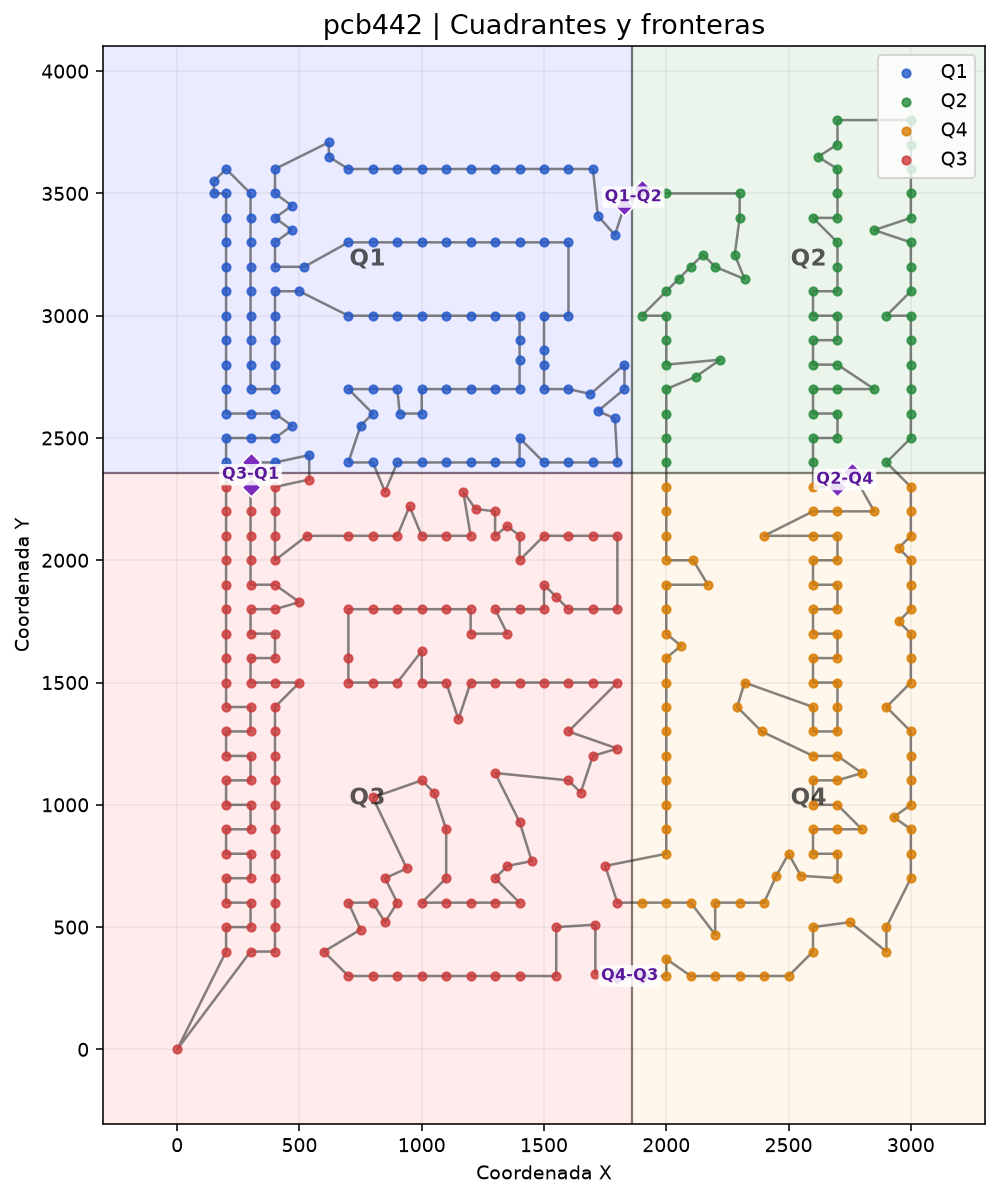
\includegraphics[width=0.70\textwidth]{Resultados_v2/PCB442_QUADRANTS.png}
\caption{Tour óptimo en \texttt{pcb442} (50\,778) coloreado por
cuadrante, con los cuatro pares de frontera elegidos.}
\label{fig:pcb442-quad}
\end{figure}

\begin{figure}
\centering
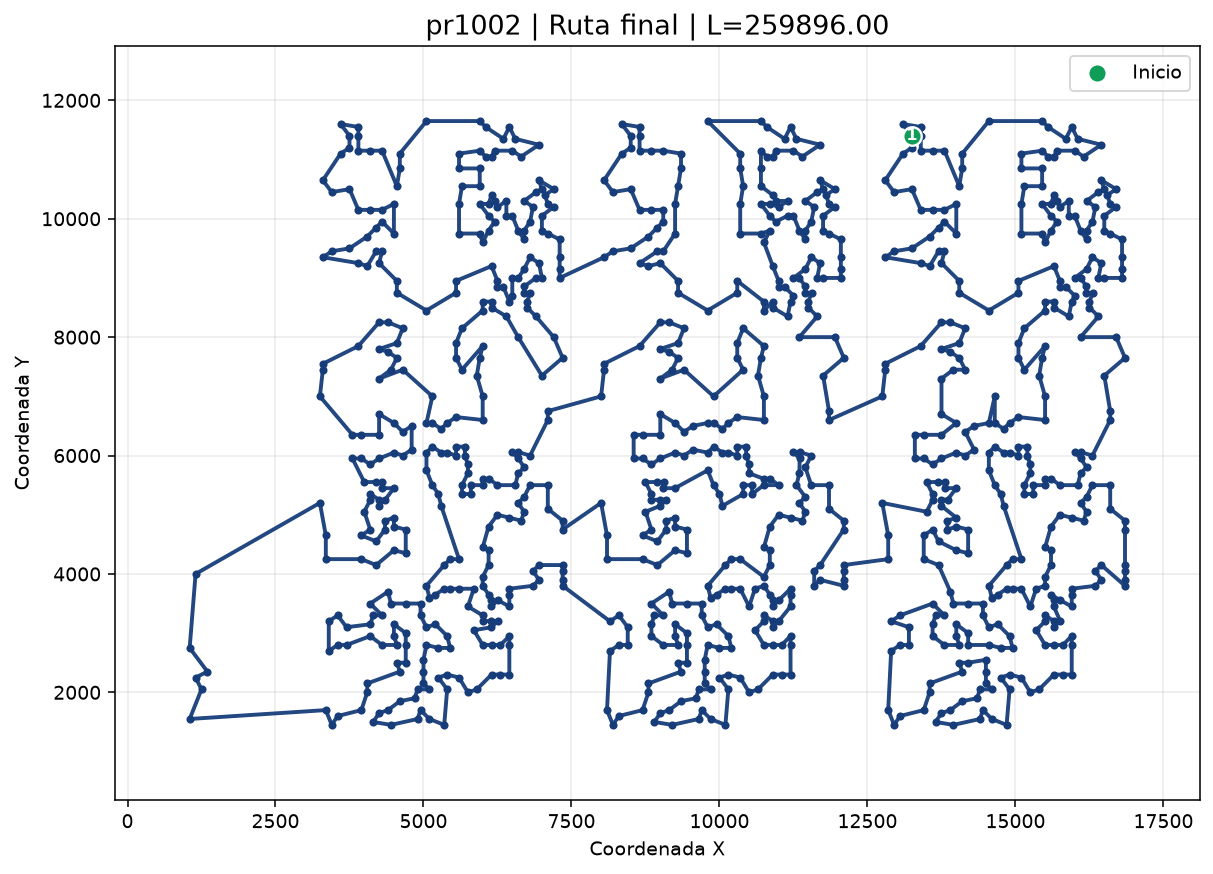
\includegraphics[width=0.70\textwidth]{Resultados_v2/PR1002.png}
\caption{Tour encontrado en \texttt{pr1002} en una sola ejecución
(259\,896, 0.329\% sobre la BKS).}
\label{fig:pr1002-route}
\end{figure}

\subsection{Aporte de la construcción}
\label{sec:ablation}

Para aislar la construcción, la reemplazamos y dejamos todo lo demás
fijo: cada variante va seguida exactamente de la misma búsqueda local y
el mismo ILS, con las mismas listas de candidatos, temperatura, ventana,
regla de parada y semillas.
\begin{itemize}
  \item \textbf{Aleatorio + ILS}: una permutación aleatoria, un piso sin
    información de construcción;
  \item \textbf{Vecino más cercano + ILS}: la línea base clásica,
    partiendo de la primera ciudad;
  \item \textbf{Partición (sin FC) + ILS}: los cuadrantes de la caja
    envolvente, cada uno recorrido con un camino abierto libre (vecino
    más cercano más 2-opt) y concatenados en el orden
    $Q_1\!\to\!Q_2\!\to\!Q_4\!\to\!Q_3$, orientando cada camino para
    empalmar con el anterior; sin pares de frontera;
  \item \textbf{Conectividad de fronteras + ILS}: los mismos cuadrantes,
    con el mejor par de cada frontera como anclas; una sola partición y
    una sola combinación de fronteras;
  \item \textbf{GSPH-FC (completo)}: portafolio de particiones, los 3
    mejores pares por frontera, combinaciones y embudo.
\end{itemize}

\begin{table}
\caption{Ablación de la construcción en las 63 instancias de TSPLIB con
$n\le 2\,000$ (5 ejecuciones cada una, semillas 1000--1004, 315
ejecuciones por variante). Cada variante va seguida de la misma búsqueda
local y el mismo ILS. Los GAP (\%) son promedios sobre instancias: del
tour inicial, del primer óptimo local (BL), del mejor de los cinco tours
finales y de todos los tours finales. Los aciertos son tours finales en
la BKS. Los tiempos se midieron mientras otros experimentos compartían la
máquina y solo son comparables dentro de la tabla.}
\label{tab:ablation-constr}
\centering\scriptsize
\begin{tabular}{@{}lrrrrrr@{}}
\toprule
\textbf{Construcción} & \textbf{GAP inicial} & \textbf{GAP BL} & \textbf{GAP mejor} & \textbf{GAP prom.} & \textbf{Aciertos} & \textbf{Tiempo (s)}\\
\midrule
Aleatorio + ILS                  & 1815.62 & 6.17 & 0.037 & 0.117 & 165/315 & 1.31 \\
Vecino más cercano + ILS         &   24.71 & 4.43 & 0.074 & 0.140 & 168/315 & 1.29 \\
Partición (sin FC) + ILS         &   23.50 & 5.44 & 0.040 & 0.101 & 170/315 & 1.27 \\
Conectividad de fronteras + ILS  &   13.84 & 6.27 & 0.038 & 0.096 & 172/315 & 1.36 \\
\textbf{GSPH-FC (completo)}      & \textbf{9.95} & \textbf{4.37} & \textbf{0.034} & \textbf{0.080} & \textbf{190/315} & 1.38 \\
\midrule
& \multicolumn{2}{c}{$n\le 300$ (36)} & \multicolumn{2}{c}{$301\le n\le 800$ (12)} & \multicolumn{2}{c}{$801\le n\le 2\,000$ (15)}\\
\cmidrule(lr){2-3}\cmidrule(lr){4-5}\cmidrule(lr){6-7}
& \textbf{GAP prom.} & \textbf{Aciertos} & \textbf{GAP prom.} & \textbf{Aciertos} & \textbf{GAP prom.} & \textbf{Aciertos}\\
\midrule
Aleatorio + ILS                  & 0.030 & 152/180 & 0.106 & 11/60 & 0.333 & 2/75 \\
Vecino más cercano + ILS         & 0.026 & 161/180 & 0.271 &  7/60 & 0.309 & 0/75 \\
Partición (sin FC) + ILS         & 0.046 & 152/180 & 0.083 & 13/60 & \textbf{0.249} & 5/75 \\
Conectividad de fronteras + ILS  & 0.021 & 160/180 & 0.079 & 11/60 & 0.289 & 1/75 \\
\textbf{GSPH-FC (completo)}      & \textbf{0.000} & \textbf{174/180} & \textbf{0.078} & \textbf{15/60} & 0.274 & 1/75 \\
\bottomrule
\end{tabular}
\end{table}

La Tabla~\ref{tab:ablation-constr} muestra dos cosas. Primero, la
construcción mejora claramente el punto de partida: el tour inicial de
GSPH-FC completo queda 9.95\% sobre la BKS, frente a 24.71\% del vecino
más cercano y 23.50\% de la partición sin pares de frontera. Elegir solo
los pares de frontera baja el GAP inicial a 13.84\%, y el portafolio con
combinaciones de fronteras lo deja bajo 10\%. Segundo, el ILS cierra la
mayor parte de la brecha restante sea cual sea el inicio: incluso los
tours aleatorios terminan con un GAP promedio de 0.117\%. Sobre las 63
instancias el método completo queda primero, con un GAP promedio de
0.080\% frente a 0.096--0.140\% y 190 aciertos de la BKS frente a
165--172, con aproximadamente el mismo tiempo total. Las diferencias son
pequeñas. Una prueba de rangos con signo de Wilcoxon sobre los GAP
promedio por instancia encuentra que el método completo es
significativamente mejor que el inicio aleatorio ($p=0.029$, 37
instancias sin empate), pero no que el vecino más cercano ($p=0.11$), la
partición sin pares de frontera ($p=0.46$) ni la conectividad de
fronteras con una sola combinación ($p=0.51$). El desglose por tamaño
tiene dos salvedades. Para $n\le 300$ el método completo puede pulir dos
finalistas y gasta cerca del doble de tiempo que las demás variantes
(0.22~s frente a 0.12~s). Para $801\le n\le 2\,000$ la partición sin
pares de frontera tiene el menor GAP promedio.

\subsection{Convergencia en el tiempo}
\label{sec:convergence}

La ablación deja una pregunta abierta: ¿por qué un tour inicial más del
doble de bueno (9.95\% frente a 23.50\% sobre la BKS) se traduce en una
diferencia tan pequeña al final? O bien el ILS borra rápidamente las
diferencias entre tours iniciales, o bien el inicio geométrico ayuda
sobre todo en las primeras etapas de la búsqueda. Para distinguir entre
ambas, registramos el mejor tour encontrado en el tiempo para tres
construcciones seguidas del mismo ILS: vecino más cercano, partición sin
pares de frontera y GSPH-FC completo. Usamos ocho instancias de 200 a
1\,889 ciudades con distinta estructura espacial, y 5 ejecuciones cada
una. El reloj parte después de construir la matriz de distancias y las
listas de candidatos, porque ese preprocesamiento es idéntico para todas
las variantes. La Figura~\ref{fig:convergence} muestra las curvas y la
Tabla~\ref{tab:convergence} las resume en fracciones fijas del tiempo de
ejecución.

\begin{figure}
\centering
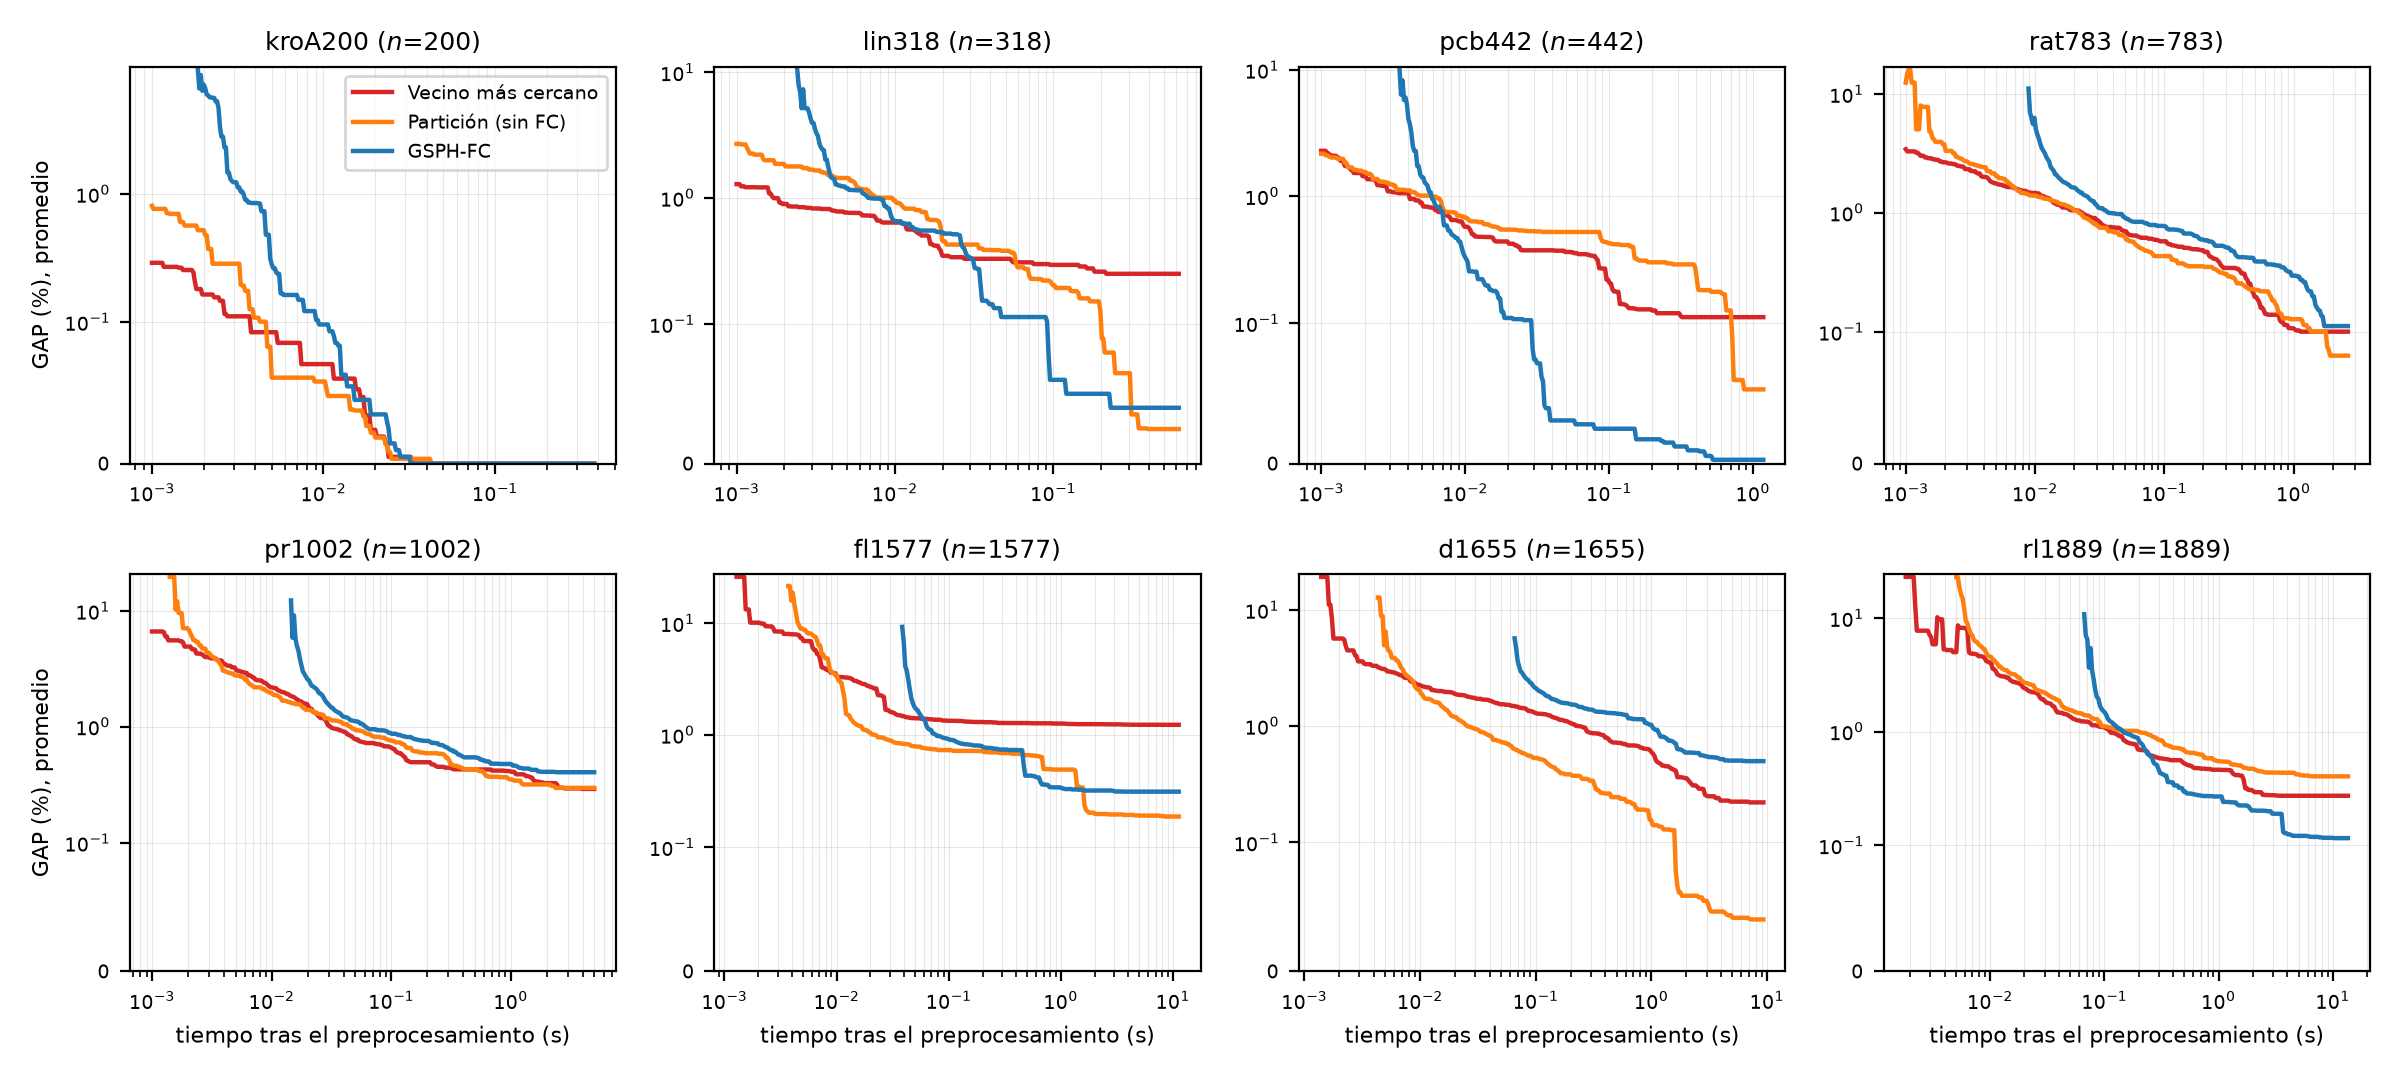
\includegraphics[width=\textwidth]{Resultados_v3/convergencia_es.png}
\caption{Mejor GAP encontrado frente al tiempo tras el preprocesamiento
(escalas logarítmicas; promedio de 5 ejecuciones), para tres
construcciones seguidas del mismo ILS.}
\label{fig:convergence}
\end{figure}

\begin{table}
\caption{GAP promedio (\%) sobre las ocho instancias de la
Fig.~\ref{fig:convergence} en fracciones fijas del tiempo promedio de
GSPH-FC en cada instancia (0.34--9.1~s).}
\label{tab:convergence}
\centering\scriptsize
\begin{tabular}{@{}lrrrrr@{}}
\toprule
\textbf{Construcción + ILS} & \textbf{1\%} & \textbf{3\%} & \textbf{10\%} & \textbf{30\%} & \textbf{100\%}\\
\midrule
Vecino más cercano      & 0.993 & 0.684 & 0.502 & 0.358 & 0.311 \\
Partición (sin FC)      & \textbf{0.972} & \textbf{0.604} & \textbf{0.414} & 0.259 & \textbf{0.152} \\
GSPH-FC (completo)      & 2.307 & 0.690 & 0.468 & \textbf{0.255} & 0.186 \\
\bottomrule
\end{tabular}
\end{table}

La segunda explicación no se sostiene, y la primera sí. La construcción
completa no tiene una ventaja temprana: parte atrás. Evalúa varias
particiones y combinaciones de fronteras y lleva varios tours iniciales a
un óptimo local antes de que empiece el ILS. Por eso su primer tour
completo aparece a los 12~ms aproximadamente (mediana), frente a 0.5~ms
del vecino más cercano y 1.3~ms de la partición, y al 1\% del tiempo de
ejecución su GAP promedio es 2.31\% frente a cerca de 1\% de los otros
dos. Después, el ILS borra la mayor parte de las diferencias: al 10\%
del tiempo las tres variantes quedan a menos de 0.1 puntos entre sí en
promedio. El orden final depende de la instancia. La construcción
completa termina mejor en \texttt{pcb442} y \texttt{rl1889} y empata en
\texttt{kroA200} y \texttt{lin318}. Es peor que la partición sin pares
de frontera en \texttt{fl1577} (agrupada) y \texttt{d1655} (de
perforación). El vecino más cercano, a su vez, se queda en 1.23\% en
\texttt{fl1577}, donde ambos inicios geométricos terminan en 0.2--0.3\%.
Con cinco ejecuciones por instancia estas diferencias tienen ruido. Sin
embargo, junto con la Tabla~\ref{tab:ablation-constr}, indican que el
valor de un inicio geométrico está menos en la velocidad que en evitar
zonas pobres del espacio de búsqueda, como hace el vecino más cercano en
instancias agrupadas. También muestran que el portafolio completo paga un
costo inicial que solo se compensa en algunas instancias.

\subsection{Componentes del motor de búsqueda}
\label{sec:engine-ablation}

La Tabla~\ref{tab:ablation} aísla la regla de aceptación en seis
instancias elegidas por su dificultad (5 ejecuciones cada una, semillas
1000--1004). Con $T=0$ la búsqueda acepta solo perturbaciones que no
empeoran. En \texttt{kroE100} todas las ejecuciones terminan entonces en
el mismo óptimo local (22\,106, 0.172\%), y tres millones de
perturbaciones adicionales no logran salir de él. Con $T=0.2\,\bar d$
las cinco ejecuciones alcanzan la BKS, y el GAP promedio de
\texttt{rat783} baja de 0.509\% a 0.111\%. La ventana de perturbación
también importa: con una ventana fija de 50 posiciones, \texttt{d1655}
se estancaba en 1.671\% en todas las ejecuciones, mientras que la
ventana dependiente del tamaño $W(n)$ redujo su mejor GAP a 0.325\%
incluso sin la regla de aceptación.

\begin{table}
\caption{Efecto de la temperatura de aceptación (5 ejecuciones, semillas
1000--1004).}
\label{tab:ablation}
\centering\scriptsize
\begin{tabular}{@{}lrrrrrrr@{}}
\toprule
& & \multicolumn{3}{c}{$T=0$ (solo no empeora)} & \multicolumn{3}{c}{$T=0.2\,\bar d$} \\
\cmidrule(lr){3-5}\cmidrule(lr){6-8}
\textbf{Instancia} & $n$ & \textbf{GAP mejor} & \textbf{GAP prom.} & \textbf{Tiempo} & \textbf{GAP mejor} & \textbf{GAP prom.} & \textbf{Tiempo} \\
\midrule
kroE100 &  100 & 0.172 & 0.172 & 0.07 & \textbf{0.000} & 0.000 & 0.09 \\
lin318  &  318 & \textbf{0.000} & 0.054 & 0.28 & \textbf{0.000} & 0.040 & 0.33 \\
pcb442  &  442 & \textbf{0.000} & 0.016 & 0.48 & \textbf{0.000} & 0.003 & 0.59 \\
rat783  &  783 & 0.261 & 0.509 & 1.15 & 0.023 & 0.111 & 1.90 \\
pr1002  & 1002 & 0.294 & 0.459 & 1.94 & 0.326 & 0.404 & 2.22 \\
d1655   & 1655 & 0.325 & 0.653 & 4.50 & 0.034 & 0.499 & 5.26 \\
\midrule
\textit{Promedio} & & 0.175 & 0.311 & 1.40 & 0.064 & 0.176 & 1.73 \\
\bottomrule
\end{tabular}
\end{table}

El diseño del motor también explica los tiempos de ejecución. Una
implementación anterior con la misma construcción, pero con una búsqueda
sin compilar, copias del tour completo al rechazar y un presupuesto fijo
de 5--30~s por ejecución, realizaba unas 290 iteraciones de ILS por
segundo en \texttt{pcb442}; el motor localizado realiza unas 420 mil. En
las 37 instancias en que se corrió la implementación anterior, esta
alcanzaba la BKS en 22 con 14.65~s por ejecución en promedio, mientras
que GSPH-FC la alcanza en las 37 con 0.23~s por ejecución, unas 65 veces
más rápido. Ambas se midieron en la misma máquina.

\subsection{Sensibilidad de parámetros}
\label{sec:sensitivity}

La Tabla~\ref{tab:sensitivity} varía un parámetro a la vez en torno a su
valor por defecto. Para no ajustar sobre una muestra estrecha, usamos 16
instancias de 100 a 1\,889 ciudades con distintas distribuciones
espaciales: uniformes aleatorias (\texttt{kroA100}, \texttt{ch150},
\texttt{kroB200}, \texttt{rd400}), agrupadas (\texttt{fl417},
\texttt{fl1400}), de perforación y circuitos impresos (\texttt{a280},
\texttt{pcb442}, \texttt{d493}, \texttt{rat783}, \texttt{u1060},
\texttt{pcb1173}, \texttt{d1655}) y otras tres instancias de TSPLIB
(\texttt{pr1002}, \texttt{vm1748}, \texttt{rl1889}). Cada variante se
corre 5 veces (semillas 1000--1004) en cada instancia.

\begin{table}
\caption{Sensibilidad de parámetros, uno a la vez, en 16 instancias (5
ejecuciones cada una, 80 ejecuciones por variante). El GAP prom. (\%) se
promedia sobre todas las instancias y sobre las ocho con $n\le 500$ y las
ocho con $n>500$. Los aciertos son ejecuciones en la BKS. Los tiempos se
midieron mientras otros experimentos compartían la máquina y solo son
comparables dentro de la tabla.}
\label{tab:sensitivity}
\centering\scriptsize
\begin{tabular}{@{}llrrrrr@{}}
\toprule
& & \multicolumn{3}{c}{\textbf{GAP prom.}} & & \\
\cmidrule(lr){3-5}
\textbf{Parámetro} & \textbf{Valor} & \textbf{Todas} & $n\le 500$ & $n>500$ & \textbf{Aciertos} & \textbf{Tiempo (s)}\\
\midrule
\multicolumn{2}{@{}l}{\textit{Por defecto} ($k{=}3$, portafolio, $T{=}0.2\bar d$, $n/8$, $300n$)} & 0.149 & 0.027 & 0.270 & 29/80 & 2.56 \\
\midrule
Pares por frontera $k$        & 1 & 0.152 & 0.042 & 0.263 & 29/80 & 2.64 \\
                              & 5 & 0.169 & 0.068 & 0.270 & 27/80 & 2.55 \\
Portafolio de particiones     & solo caja & 0.177 & 0.089 & 0.264 & 22/80 & 2.39 \\
Temperatura $T/\bar d$        & 0   & 0.257 & 0.068 & 0.445 & 29/80 & 2.02 \\
                              & 0.1 & 0.177 & 0.039 & 0.315 & 24/80 & 2.40 \\
                              & 0.4 & 0.164 & 0.047 & 0.280 & 19/80 & 2.04 \\
Divisor de ventana ($n/\cdot$)& 4  & 0.152 & 0.023 & 0.281 & 28/80 & 3.18 \\
                              & 16 & 0.241 & 0.024 & 0.458 & 24/80 & 2.20 \\
Factor de estancamiento ($\cdot\,n$) & 100  & 0.209 & 0.039 & 0.379 & 19/80 & 0.93 \\
                              & 1000 & 0.110 & 0.020 & 0.201 & 33/80 & 7.27 \\
\bottomrule
\end{tabular}
\end{table}

La mayoría de las diferencias aparece en las instancias más grandes.
Para $n\le 500$ casi todas las variantes terminan a pocas centésimas de
porcentaje de la BKS, así que la elección de parámetros importa sobre
todo para $n>500$. Se desprenden cuatro conclusiones.

\emph{Aceptación y ventana.} Son los parámetros que más necesitan estar
bien elegidos. Sin la regla de aceptación ($T=0$), el GAP promedio para
$n>500$ sube de 0.270\% a 0.445\%, y el valor por defecto es mejor en 10
de las 16 instancias y peor en solo 2. Los valores de $T/\bar d$ entre
0.1 y 0.4 son todos razonables, y 0.2 tiene el menor promedio. Una
ventana de $n/16$ es claramente demasiado pequeña (0.458\% para $n>500$,
y 0.41\% frente a 0.10\% en las instancias agrupadas). Una ventana de
$n/4$ iguala al valor por defecto en calidad, pero toma cerca de 24\% más
tiempo, así que $n/8$ es el mejor compromiso.

\emph{Pares de frontera.} La cantidad de pares por frontera casi no
importa. Con cinco pares, el resultado promedio es idéntico al del valor
por defecto en 15 de las 16 instancias, porque solo se ensamblan las tres
a cinco combinaciones mejor ubicadas. Con un solo par, el resultado
empeora en 6 instancias y mejora en 3.

\emph{Portafolio de particiones.} Su efecto depende de la estructura
espacial de la instancia. Con solo la partición de la caja envolvente,
las instancias agrupadas mejoran notablemente (0.007\% frente a 0.104\%),
mientras que las de perforación y las demás empeoran, y la variante
alcanza la BKS con menos frecuencia (22 frente a 29 ejecuciones). Esto
coincide con las curvas de convergencia, donde la partición única sin
pares de frontera también fue mejor en \texttt{fl1577}. Por lo tanto, el
portafolio es un valor por defecto razonable, no una mejora universal.

\emph{Factor de estancamiento.} Es un control puro entre tiempo y
calidad, no un parámetro de ajuste. Un factor de $1000n$ mejora el GAP
promedio de 0.149\% a 0.110\% y es mejor que el valor por defecto en 10
instancias y peor en ninguna, pero toma 2.8 veces más tiempo. Un factor
de $100n$ es cerca de 2.7 veces más rápido, con 0.209\%. El valor por
defecto $300n$ es un punto intermedio. Un usuario con un presupuesto de
tiempo mayor debería subir este factor en vez de cambiar cualquier otro
parámetro.

\subsection{Comparación con LKH}
\label{sec:lkh}

LKH~\cite{helsgaun2000effective,helsgaun2017extension} es la heurística
de referencia para el TSP simétrico. Corrimos LKH-3 (versión 3.0.8,
mediante el paquete de Python \texttt{elkai}, que incluye el código C
original) en las mismas instancias y semillas con dos configuraciones:
con sus parámetros por defecto (una ejecución de $n$ intentos por
semilla) y con un límite de tiempo igual al tiempo promedio por ejecución
de GSPH-FC en esa instancia. LKH no cuenta su preprocesamiento (ascenso
por subgradiente para los candidatos por $\alpha$-cercanía) dentro de ese
límite, así que reportamos el tiempo total medido. Cada tour de LKH se
validó y su largo se recalculó con \texttt{EUC\_2D}.

\begin{table}
\caption{GSPH-FC frente a LKH-3 en las 63 instancias de TSPLIB con
$n\le 2\,000$. GSPH-FC: 10 ejecuciones por instancia. LKH: 3 ejecuciones
por instancia (semillas 1000--1002), con parámetros por defecto y con un
límite de tiempo igual al tiempo promedio de GSPH-FC. El GAP prom. (\%) y
el tiempo (s) son promedios sobre instancias; los aciertos son
ejecuciones en la BKS.}
\label{tab:lkh}
\centering\scriptsize
\begin{tabular}{@{}lrrrrrrrrr@{}}
\toprule
& \multicolumn{3}{c}{\textbf{GSPH-FC}} & \multicolumn{3}{c}{\textbf{LKH por defecto}} & \multicolumn{3}{c}{\textbf{LKH, mismo tiempo}}\\
\cmidrule(lr){2-4}\cmidrule(lr){5-7}\cmidrule(lr){8-10}
\textbf{Rango} & \textbf{GAP} & \textbf{Aciertos} & \textbf{Tiempo} & \textbf{GAP} & \textbf{Aciertos} & \textbf{Tiempo} & \textbf{GAP} & \textbf{Aciertos} & \textbf{Tiempo}\\
\midrule
$n\le 300$ (36)           & 0.001 & 342/360 & 0.22 & 0.001 & 105/108 &  0.12 & 0.001 & 105/108 & 0.10 \\
$301\le n\le 800$ (12)    & 0.081 &  25/120 & 0.82 & 0.010 &  31/36  &  2.06 & 0.010 &  30/36  & 0.88 \\
$801\le n\le 2\,000$ (15)& 0.301 &   1/150 & 3.63 & 0.041 &  21/45  & 14.55 & 0.073 &  16/45  & 4.52 \\
\midrule
\textit{Todas} (63)       & 0.088 & 368/630 & 1.14 & 0.012 & 157/189 &  3.93 & 0.020 & 151/189 & 1.30 \\
\bottomrule
\end{tabular}
\end{table}

LKH es la heurística más fuerte (Tabla~\ref{tab:lkh}), como se espera de
un método maduro basado en candidatos por $\alpha$-cercanía y
movimientos secuenciales 5-opt. Para $n\le 300$ ambos métodos alcanzan
la BKS en casi todas las ejecuciones, y LKH necesita cerca de la mitad
del tiempo. En el rango intermedio LKH logra un GAP promedio de 0.010\%
frente a 0.081\% de GSPH-FC, tanto con sus parámetros por defecto (2.5
veces más lento que GSPH-FC) como limitado al tiempo de GSPH-FC. Para
$801\le n\le 2\,000$ la diferencia crece: 0.041\% para LKH con sus
parámetros por defecto, que tardan cuatro veces más, 0.073\% con el mismo
tiempo y 0.301\% para GSPH-FC. Sobre las 63 instancias, GSPH-FC tiene un
GAP promedio menor que LKH en solo tres (\texttt{ch150}, \texttt{lin318}
y \texttt{fl1577} con igual tiempo), empata en 29 y es peor en el resto.

% ================================================================
\section{Discusión}
\label{sec:discussion}
% ================================================================

\paragraph{Qué aporta cada fase.} La ablación y las curvas de
convergencia dan una imagen coherente. La construcción condicionada por
fronteras produce los mejores tours iniciales y, al final, la mayor
cantidad de aciertos de la BKS y el menor GAP promedio sobre 63
instancias. Sin embargo, el ILS localizado explica la mayor parte de la
calidad final, y borra rápido las diferencias entre tours iniciales:
incluso los tours aleatorios terminan a menos de 0.12\% de la BKS en
promedio. El beneficio de un inicio geométrico es sobre todo de
robustez. Partir de la estructura de cuadrantes evita zonas pobres, como
el 1.23\% en que se estanca el vecino más cercano en \texttt{fl1577}, más
que dar una ventaja temprana. El portafolio completo, que construye y
pule varios tours iniciales, tiene un costo inicial de unos 10~ms y se
compensa en algunas instancias (\texttt{pcb442}, \texttt{rl1889}) pero no
en otras (\texttt{fl1577}, \texttt{d1655}). Esto sugiere una variante
más liviana, con una sola partición y pares de frontera, para contextos
donde se necesita un tour utilizable en milisegundos. Como las
iteraciones cuestan microsegundos, el motor alcanza la BKS en todas las
instancias de hasta 300 ciudades en mucho menos de un segundo.
Consideramos que separar con honestidad ambos aportes es parte del
resultado: la idea geométrica es sólida e interpretable, pero no se le
debe atribuir una calidad que entrega el motor de búsqueda.

\paragraph{Posicionamiento.} GSPH-FC no compite con LKH en calidad de
solución por encima de unos cientos de ciudades, y no afirmamos lo
contrario. Su valor está en otros aspectos: una construcción que se puede
leer y dibujar, una base de código corta en Python con núcleos
compilados, resultados a pocas décimas de porcentaje del óptimo en
segundos y un solo parámetro, $S(n)$, que mueve al método a lo largo de
su curva entre tiempo y calidad (Sección~\ref{sec:sensitivity}).

\paragraph{Limitaciones.} Primero, por encima de unas 10\,000 ciudades
la representación con arreglos hace que cada inversión cueste $O(n)$,
las ejecuciones terminan en el tope de 60~s antes del estancamiento y la
matriz densa de distancias se convierte en el cuello de botella de
memoria. Segundo, las instancias muy agrupadas, como \texttt{fl3795},
muestran una gran dispersión entre ejecuciones, lo que sugiere que las
perturbaciones que cruzan entre grupos están subrepresentadas. Tercero,
los cuadrantes alineados con los ejes pueden no ajustarse bien a
instancias alargadas o agrupadas en diagonal. Cuarto, la ablación y la
comparación con LKH cubren instancias de hasta 2\,000 ciudades con 3--5
ejecuciones cada una; estudios más amplios precisarían las pequeñas
diferencias entre construcciones. Los pasos siguientes naturales son un
movimiento de profundidad variable (tipo Or-3opt o Lin--Kernighan)
dentro del mismo esquema de inversiones, listas doblemente enlazadas de
dos niveles con distancias calculadas al vuelo para las instancias más
grandes, orientaciones de partición adaptativas y costos asimétricos
provenientes de redes viales reales.

% ================================================================
\section{Conclusiones}
\label{sec:conclusions}
% ================================================================

GSPH-FC combina una construcción geométrica en la que las conexiones
entre cuadrantes se deciden antes de rutear los cuadrantes con un ILS
localizado cuyas iteraciones cuestan microsegundos. En 77 instancias de
TSPLIB alcanza la BKS en 44, incluidas todas las de $n\le 300$ en menos
de medio segundo, y se mantiene a menos de 0.60\% de la BKS hasta 6\,000
ciudades. Medir las dos fases por separado muestra que la conectividad
de fronteras entrega los mejores tours iniciales y los resultados más
consistentes, mientras que el ILS localizado explica la mayor parte de
la calidad final. Las curvas de convergencia muestran que esta ventaja no
es temprana: el ILS borra la mayor parte de las diferencias entre tours
iniciales dentro de la primera décima de la ejecución, y un inicio
geométrico ayuda sobre todo a evitar zonas pobres en instancias
agrupadas. GSPH-FC iguala a LKH-3 en instancias pequeñas, pero no por
encima de 300 ciudades, lo que lo sitúa como una alternativa liviana e
interpretable más que como un reemplazo. Todas las tablas y figuras se
pueden reproducir con los scripts que acompañan el trabajo.

% REVISIÓN CIEGA: agradecimientos ocultos
%
% RESTAURAR ANTES DE LA VERSIÓN FINAL:
%\begin{credits}
%\subsubsection{\ackname}
%Los autores agradecen al equipo docente del curso de Heurísticas de la
%Universidad Andrés Bello por su orientación y apoyo material durante el
%desarrollo de este trabajo.
%\end{credits}

\bibliographystyle{splncs04}
\bibliography{bibliografia}

\end{document}
